\setlength{\footskip}{8mm}

\chapter{Introduction} 

\textit{This dissertation explores the possibilities and develops
algorithms for modeling human behaviors and detecting anomalies
without requiring large databases of training data. In this chapter, I
discuss the background of, and motivation for my work. Additionally, 
I review real-world surveillance systems, present the contributions of 
the work, and provide an outline of this dissertation.}

\section{Background and Motivation}

Due to the increase in demand for video surveillance in public areas,
video surveillance is becoming ubiquitous in our lives. It becomes
increasingly important for preventing and responding to terroristic 
threats and other criminal activities. However, the resulting proliferation of
surveillance cameras is making it increasingly difficult to monitor
all channels continuously. Human monitoring is therefore becoming
increasingly expensive and ineffective as the torrent of video data
increases. For instance, in a CCTV monitoring room (see
Figure \ref{fig:monitoring}), security operators are required to
monitor 24 hours a day and be ready to take action when an alarm
occurs. Security will be enhanced if there is an intelligent
surveillance system able to perform filtering, archive ``normal''
events, and automatically raise alarms for possible ``abnormal''
events or presenting such events to human security personnel for
consideration as a security threat. The problems to consider in a
surveillance system include pedestrian detection and tracking,
unattended object detection, human behavior modeling, and anomaly
detection.

\begin{figure}[t]
    \centering
    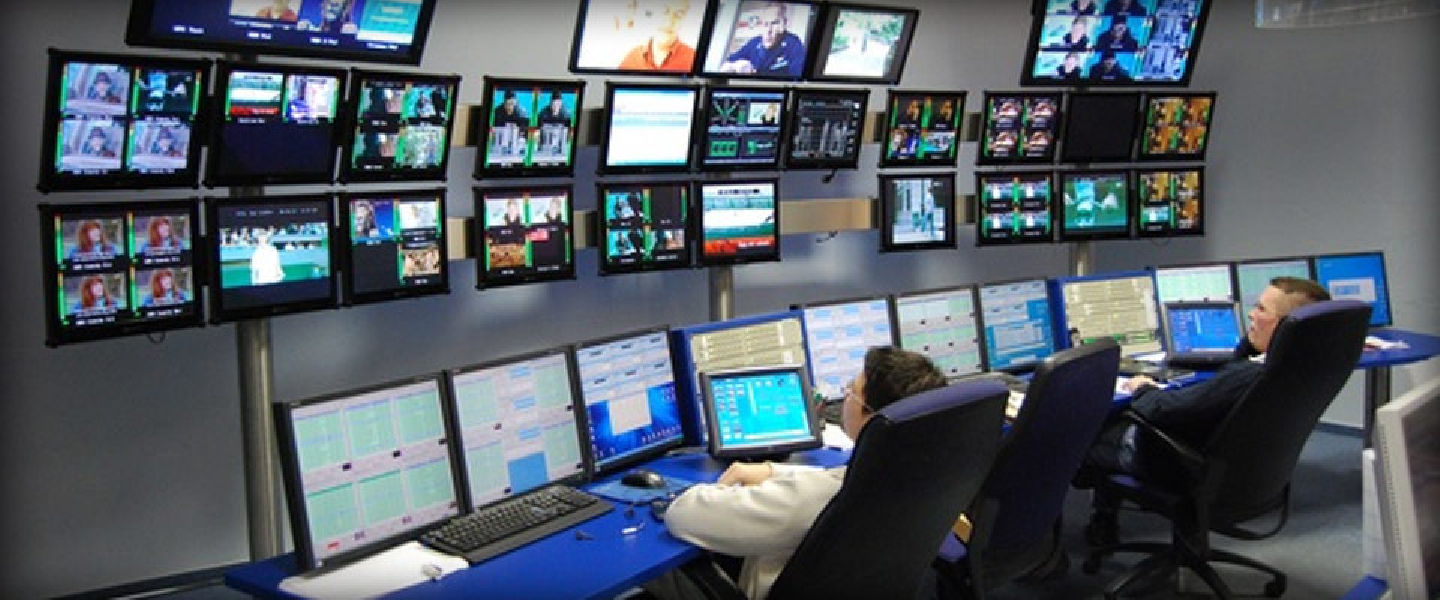
\includegraphics[width=5in]{figures/monitoring}
    \caption[CCTV monitoring room.]{\small CCTV monitoring
        room. Reprinted from the Twenty First Security Web site
        (\url{http://www.twentyfirstsecurity.com.au/}).}
    \label{fig:monitoring}
\end{figure}

Human behavior understanding is one of the most intricate and complex facets of
intelligent video surveillance. 
Clearly, behavioral understanding can be problematic because it requires 
considerable time to study each individual subject, and often cannot 
predict ``one-time'' malicious behavior before it happens.
The problem is difficult and
remains unsolved, due to the wide range of activities possible in any
given context and the large amount of variability within any
particular activity.

One limitation of much of the existing work is that it learns in batch
mode and creates separate models, which remain static once trained,
for each distinct class of behavior. It may have an advantage in
explaining data that are well-defined, but it needs sufficiently large
samples of behavior patterns before training the system. Another
limitation is that the number of ``normal'' behavior patterns needs to
be known beforehand because we cannot learn a model for ``abnormal''
behavior that is rare and diverse. Therefore, we must instead detect
deviations from typical behavior.

The ambiguity of human behaviors makes the problem more challenging
since it is scene-dependent and can change over time. In particular, a
behavior considered normal in one context might be considered unusual
in another context depending on the type of behavior and where and
when it is observed. The characteristics of typical behavior also vary
from scene to scene.

Many researchers have attempted to build surveillance systems able to
interpret and understand human behaviors. However, most of the work
learns behaviors in an offline fashion and keeps the model static once
trained. This is impractical for real-time surveillance applications,
since offline training requires a great deal of computational time and
resources. In addition, the number of behaviors needs to be known
beforehand. We therefore need to find a way to initially recognize and
model each of the common behavior groups in a particular scene as well
as to incrementally learn scene-specific models as new behavior is
observed.

Many open source and commercial video surveillance products are 
available. Most of the products do not implement any intelligent
features; therefore, they cannot learn and understand the events
occurring in a scene. Moreover, a great deal of configuration must be done
before a user can deploy the system to operate in a real situation.
For instance, a user may need to define restricted zones or rules
for a specific scene.

Three main challenges for human behavior understanding and anomaly
detection are as follows.

\begin{enumerate}
    \item It is impractical to store all data in a system; therefore, we
        need an efficient approach that learns scene-specific statistical
        models of human behavior without requiring storage of large
        databases of training data.
    \item Real human behavior is sometimes ambiguous; therefore, we need to 
        keep humans such as security personnel in the loop to interpret it.
    \item Unusual behavior is rare and diverse, and it is also impractical 
        to acquire sufficient data for a good model for it; therefore, we 
        need to detect deviations from typical behavior instead.
\end{enumerate}

In this dissertation, we propose to explore, implement, and evaluate
an efficient method for automatic identification of suspicious
behavior in video surveillance data that incrementally learns
scene-specific statistical models of human behavior without requiring
storage of large databases of training data. The method is based on
hidden Markov models (HMMs) with sufficient statistics and an optimal
threshold on the likelihood of an event according to the human
behavior model.  We begin by building an initial set of models
explaining the behaviors occurring in a small bootstrap data set. The
bootstrap procedure partitions the bootstrap set into clusters then
assigns new observation sequences to clusters based on statistical
tests of HMM log likelihood scores. Cluster-specific likelihood
thresholds are learned rather than set arbitrarily. After
bootstrapping, each new sequence is used to incrementally update the
sufficient statistics of the HMM it is assigned to. Our method is an
effective solution to the problem of inducing scene-specific
statistical models useful for bringing suspicious behavior to the
attention of human security personnel.

\section{Review of State of the Art in Surveillance Systems}

We divide this section into two parts. The first part describes the 
review of open source and commercial products. The second part describes 
the review of the state of the art in surveillance systems.

\subsection{Open Source and Commercial Products}

ZoneMinder (ZM; Coombes, 2007)\nocite{zoneminder} is an open source
video surveillance system for Linux. It has been released under the
terms of the GNU general public license (GPL). ZM supports both IP
cameras and USB cameras. Figure \ref{fig:zm-webcam} shows an example
of a scene captured by an IP camera and a USB camera. The system
consists of many independent modules including motion detection.  Each
component is designed to use as few resources as possible, maximizing
the efficiency of the machine. It provides a PHP-based Web interface
that allows us to control the cameras and monitor a scene from
anywhere. Besides controlling and monitoring, we can also review,
archive, or delete the events through its Web interface.

\begin{figure}[t]
  \begin{center}
    \subfloat[]{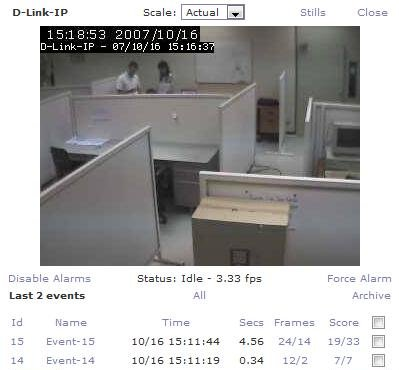
\includegraphics[scale=0.6]{figures/zm-webcam01.jpg}
    \label{fig:zm-webcam01}}
    \hspace{0.1in}
    \subfloat[]{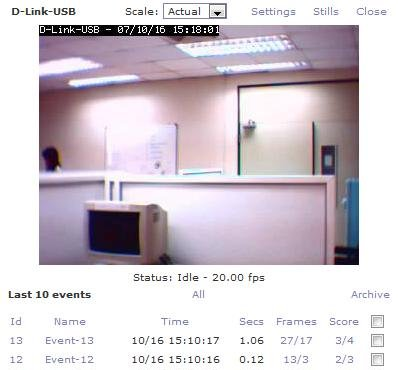
\includegraphics[scale=0.6]{figures/zm-webcam02.jpg}
    \label{fig:zm-webcam02}}
  \end{center}
  \caption[Example of a scene captured by ZoneMinder.]{\small Example
    of a scene captured by (a) an IP camera and (b) a USB camera from
    ZoneMinder.}
  \label{fig:zm-webcam}
\end{figure}

SecureCam \shortcite{bedecs09securecam} is an open source software project for
the Windows platform providing a friendly user interface as shown in Figure
\ref{fig:securecam}. Similar to ZoneMinder, SecureCam supports multiple cameras
and provides a few simple and fast algorithms such as motion detection. It has
e-mail and sound notification features, and it also allows users to record
video for later review.

\begin{figure}[t]
  \begin{center}
    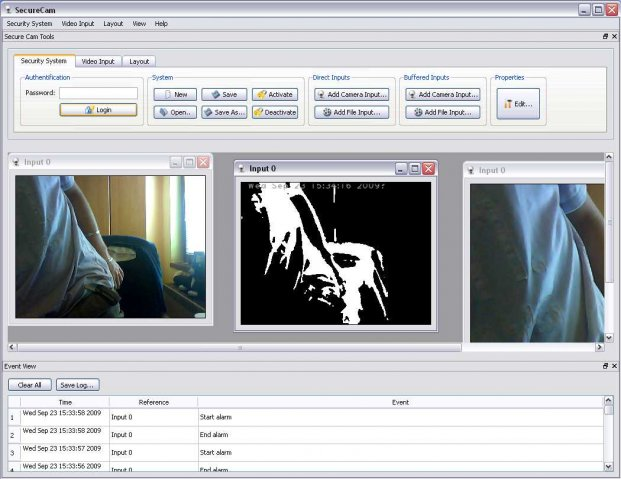
\includegraphics[width=4in]{figures/securecam.jpg}
    \caption[Screen shot of SecureCam.]{\small Screen shot of
      SecureCam. Reprinted from the SecureCam Web site
      (\url{http://sourceforge.net/projects/securecam/}).}
    \label{fig:securecam}
  \end{center}
\end{figure}

Vitamin D Video \shortcite{vitamind} is a commercial video
surveillance system. It supports USB webcams and network cameras and
provides advanced features such as creating rules for specific events.
For example, the user could create a rule to record a clip only when a
person opens a door, or the user could create a rule to notify via
email when the system senses some movement in a defined region. The
system also allows users to monitor a scene and to search for videos
of interest.  Figure \ref{fig:vitamind} shows a screen shot of the
software.

\begin{figure}[t]
  \begin{center}
    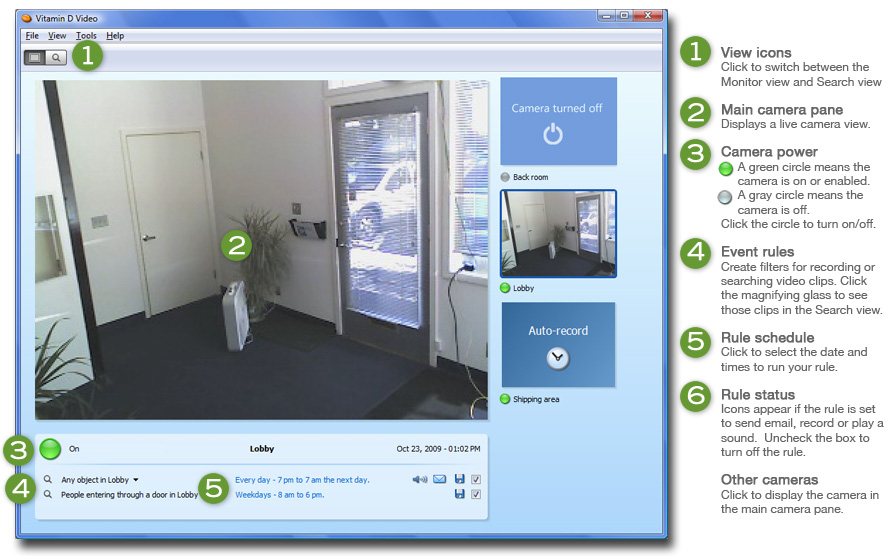
\includegraphics[width=4in]{figures/vitamind.jpg}
    \caption[Screen shot of Vitamin D Video.]{\small Screen shot of
      Vitamin D Video. Reprinted from the Vitamin D Video Web site
      (\url{http://www.vitamindinc.com/}).}
    \label{fig:vitamind}
  \end{center}
\end{figure}

It is interesting that Vitamin D Video does not use motion detection,
but rather uses people detection. It uses hierarchical temporal memory
(HTM; Hawkins, 2007)\nocite{jeff07htm} to detect people. This
algorithm attempts to apply the concept of how the brain recognizes a
human being.

Video Analytics \shortcite{dvtel} is a video surveillance software package that
includes many different modules.  Sample modules are intrusion detection, left
luggage detection, and autonomous pan-tilt-zoom (PTZ) tracking.  However, some
modules such as intrusion detection do not have any intelligent features.

SuperTrack \shortcite{supertrack} is an intelligent video surveillance
system. SuperTrack is designed for automatically analyzing and
monitoring events without the need for human attention and
interaction. This system provides automatic object detection, abnormal
behavior detection, tracking, and so on. However, it requires the user
to configure and maintain a set of alarm trigger rules in
advance. SuperTrack also supports various types of cameras such as USB
cameras and network cameras.  Figure \ref{fig:supertrack} shows a
screen shot of the system.

\begin{figure}[t]
  \begin{center}
    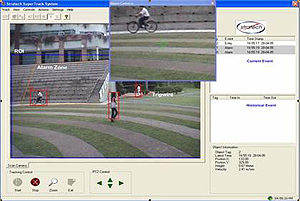
\includegraphics[width=3in]{figures/supertrack.jpg}
    \caption[Screen shot of SuperTrack.]{\small Screen shot of
      SuperTrack. Reprinted from the Stratech Web site
      (\url{http://www.stratechsystems.com/iv_supertrack.asp}).}
    \label{fig:supertrack}
  \end{center}
\end{figure}

The review on open source and commercial video surveillance 
products makes us realize the importance of and demand for human 
behavior modeling and anomaly detection. 

\subsection{State of the Art Systems}

In general, open source and commercial video surveillance products lag behind
state-of-the-art systems that are currently in development in academic
research.  Despite the vast number of systems available, most do not use much
intelligent analysis. Therefore, they cannot understand the events occurring in
a scene or learn human activities. In addition, users are required to set a
large number of configuration parameters before they can deploy a system to
operate in real-world situations.  For instance, in most commercial and open
source systems, restricted zones or rules for a scene need to be defined for
the system to operate optimally. 

There have been a number of significant advanced research with novel approaches
for visual surveillance in recent years, including automatic human activity
interpretation and wide-area surveillance to reduce maintenance costs, human
interaction, and the propensity for human error.
\shortciteA{remagnino07surveillance} introduce a journal issue that covers many
novel concepts and challenges for research on intelligent video surveillance.
One of the most challenging problems in this area is the analysis of human
activities. Various approaches can be applied to resolve the issues.  

Several researchers have proposed space-time methods, which model a human
activity using features extracted from a 3D shape in a spatio temporal vector
space, to recognize human activities from video sequence.

\shortciteA{campbell95recognition} propose a method to represent human body
movements as curves in low-dimensional ``phase spaces.'' They define a phase
space as a space that has axes representing an independent parameter of the
body based on a 3D model estimated for each frame.  The authors use this
representation to learn new movements by searching for constraints that are in
effect during the movement to be learned and not in effect during other
movements. The learned representation is used for recognizing body movements.

\shortciteA{shechtman05recognition} propose an approach to estimate motion
flows to recognize human actions using 3D space-time features. The authors
compare human activity representations in terms of their patches. They extract
a small space-time patch around every 3D point. They then represent each
space-time patch as a flow of a particular local motion. Finally, they compute
a matching score from the correlation between two patches in a template and
video at the same location.  Given a new video, the authors use a sliding
window template to search for all possible 3D patches that best match with the
template.

\shortciteA{ke07recognition} classify segmented spatio-temporal volumes
extracted from human activities using support vector machines (SVMs). The
authors use a hierarchical mean shift method to cluster colored voxels then
obtain segmented volumes. They recognize each activity by finding the best
match of a model to a subset of over-segmented spatio-temporal volumes.

As an alternative to space-time approaches, template-based approaches can be
used to represent human activities by maintaining a sequence of templates or a
set of sample action sequences. Given a new video input, the method extracts
features from the video, constructs a sequence of feature vectors, and then
measures the similarity between the constructed sequence and a sequence of
templates in the recognition process. 

\shortciteA{darrell93recognition} propose a dynamic time warping (DTW)-based
gesture recognition method using multiple template images or models to
represent the poses or the dynamics of articulated objects. They find the
correspondences between observed frames and models using the DTW algorithm.

\shortciteA{gavrila95recognition} develop a 3D model-based body part tracking
method using a DTW algorithm to recognize human actions.  Multiple cameras have
been used to obtain 3D models of a human that is represented as a stick figure
model. The authors treat each joint angle as a feature characterizing human
movement, then they use the DTW algorithm to analyze a sequence of angles and
compare the score with a pre-trained reference sequence per action.

\shortciteA{yacoob98recognition} use PCA-based modeling to represent an
activity as a linear combination of a set of eigenvectors. They compute the
projections of the activity observed from the input and action templates onto
the eigenvector basis, then they compare the projections of the two.

\shortciteA{bobick01recognition} propose a template-based human action
recognition method using human silhouette in subsequent frames to track shape
changes over time.  Each action is represented by a template that is composed
of two 2D images: a motion energy image (MEI) and a motion history image (MHI),
constructed from a sequence of foreground images. They recognize human actions
by searching for the best match between human silhouette extracted from an
image and the template, which is a pair of images, both MEI and MHI.

\shortciteA{vaswani03recognition} recognize people interaction with an airplane
using a single-layered exemplar-based sequential approach. A group activity is
represented as a shape change over time. The authors extract point objects and
construct a polygon in each frame then track those points.  Their method
extracts an activity shape from an input and measures the similarity with a
maintained model in a tangent space to recognize activities.

\shortciteA{yang10recognition-with-latent-poses} use an exemplar-based pose
representation called a ``poselet.'' A poselet is a set of patches with similar
3D pose configurations, which is expressed as a latent variable. The authors
treat the action recognition problem as inference over the latent variables. 

Statistical approaches are also widely used in activity recognition. These
approaches use statistical state-based models to recognize human activities
from historical data. Dynamic Bayesian networks (DBNs) and hidden Markov models
(HMMs) are very well-known for their effectiveness in this analysis.

\shortciteA{yamato92hmm} adopt standard HMMs to recognize tennis activities.
They extract a feature vector containing the number of foreground pixels that
are present in each cell of grid. They then treat the feature vectors as a
sequence of observations generated by an activity model, each of which is
modeled using a HMM. Given a new sequence, the authors  measure the likelihoods
of each HMM and then use the likelihood results to classify the action.

\shortciteA{bobick97recognition} use state models for gesture recognition. Each
gesture is represented by a 2D trajectory that describes the location changes
of a hand.  They compute the transition probabilities in the similar way as the
transition probabilities of HMMs. To recognize each gesture, they perform a
dynamic programming algorithm to measure the optimal matching cost between the
new observation and each gesture prototype.

\shortciteA{oliver00modeling} extend standard HMMs to the ``coupled'' HMM
(CHMM) to model human activity interactions. Since the basic HMM is
unsuitable for modeling activities involving two or more persons, the authors
then build a CHMM by coupling multiple HMM models, where each HMM models the
motion performed by one person, to model human-human interactions.

\shortciteA{cupillard02recognition} use a finite state machine to recognize
group activities. This approach is equivalent to a fully observable Markov
model. 

\shortciteA{zhong04detection} use a clustering-based similarity approach for
detecting abnormal activity in video. They evaluate the approach on several
real world surveillance videos such as a video from surveillance camera
overlooking a road adjacent to a fenced facility. 

\shortciteA{park04hierarchical} use a DBN for gesture recognition for two
interacting people. They construct a hierarchical DBN to gain an advantage of
the dependence of nature among body parts' motion.  The authors model each pose
using a set of features including locations of skin regions, maximum curvature
points, and the ratio and orientation of each body part, from the corresponding
body part to recognize gestures.

\shortciteA{vaswani05activity} use a statistical model such as a
continuous-state HMM for the configuration of a set of landmark shape dynamics
in an activity. They identify an abnormal activity defined as a change in the
shape activity model. Their approach is used in an airport scenario with people
deplaning and moving toward the terminal.

\shortciteA{park07activity} individually model body part gestures including
upper body gestures, lower body gestures, and torso translations based on the
assumption that each body part is independent of the others. Then the authors
recognize gestures using the independent sets of HMMs.

The knowledge-based approach is another well-known approach in which predefined
rules or a priori knowledge about the observed environment and video events are
used. 

\shortciteA{georis04video} built a real-time bank agency monitoring system.
Scenarios are modeled by domain expert knowledge. Then end-user feedback is
collected to improve the scenario models. 

\shortciteA{georis07surveillance} divide video events into three parts: all
objects present in the scene, sub-events involved in the event, and relations
between objects and sub-events. The authors then use a
formalism~\shortcite{vu03recognition} to model events in the scene.

\shortciteA{fusier07recognition} propose an automated video understanding
system that is able to recognize activities occurring in environments. They use
the contextual knowledge about the observed environment to build a formalism
for event modeling. The formalism is designed to allow the experts to easily
describe and define the event models.

Other related work can be found in the survey
papers\shortcite{cedras95motion,gavrila99analysis,aggarwal99motion,krueger07action,turaga08activity}
that also discuss the essential aspects of and recent research trends in
activity recognition approaches designed for human activity analysis.

%The experimental results are shown in Figure \ref{fig:zhong-work}.
%
%\begin{figure}[t]
%    \centering 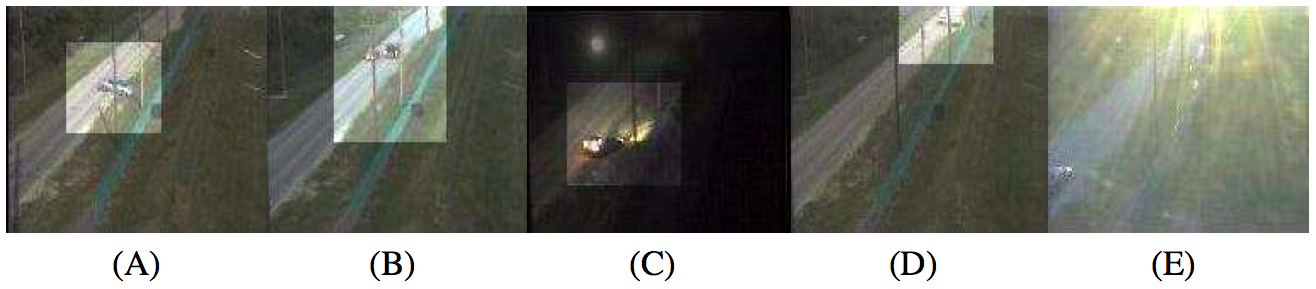
\includegraphics[width=5.5in]{figures/zhong-road-surveillance-video.png} \caption[Zhong
%    et al.'s experimental results on road surveillance video.]{Zhong
%    et al.'s experimental results on road surveillance video.  Usual
%    events consist of cars moving along the road. Correctly detected
%    unusual events include: (A) cars pulling off the road, (B) cars
%    stopping and backing up, (C) cars making U-turns and people
%    walking on the road. Undetected unusual events include: (D) cars
%    stopping on the far end, due to coarseness of the spatial
%    features. Reprinted from Zhong et al.\
%    (2004).}  \label{fig:zhong-work}
%\end{figure}

%Figure \ref{fig:georis-work} shows a scenario of a coordinated 
%bank attack of multiple robbers.
%
%\begin{figure}[t]
%    \centering
%    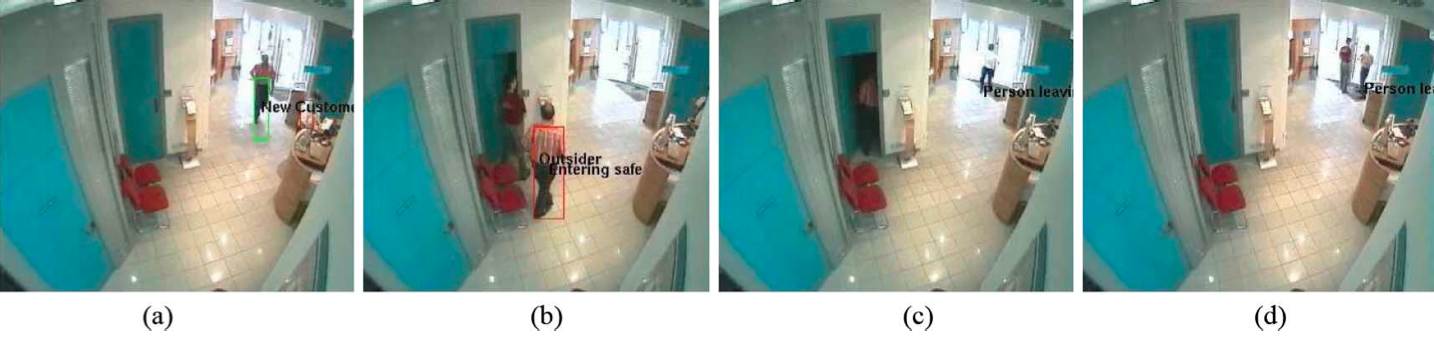
\includegraphics[width=5.5in]{figures/georis-bank-attack.png}
%    \caption[Example video of a simulated bank attack.]
%        {Example video of a simulated bank attack. (a) Person enters the bank. 
%        (b) Robber is identified to be an outsider. Robber is entering the 
%        bank safe. (c) A customer leaves the bank. (d) Robber leaves the bank. 
%        Reprinted from Turaga et al.\ (2008).\nocite{turaga08survey}}
%    \label{fig:georis-work}
%\end{figure}

%Figure \ref{fig:vaswani-work} shows an example of people 
%deplaning.
%
%\begin{figure}[t]
%    \centering
%    \subfloat[]{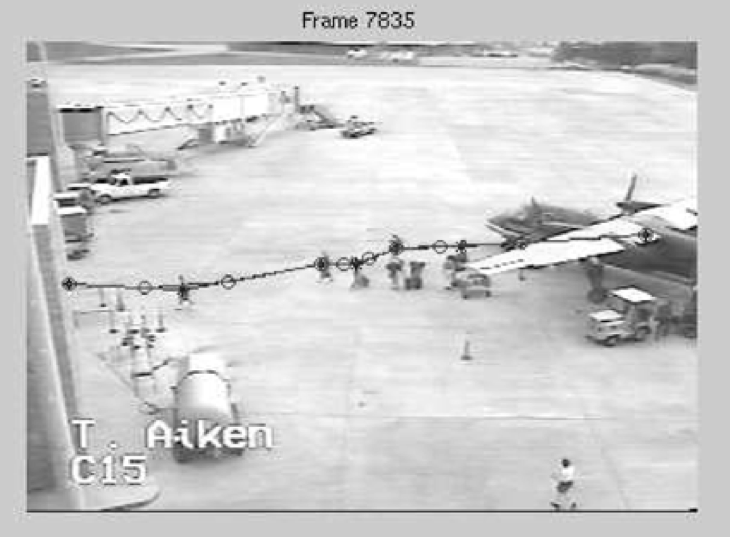
\includegraphics[width=2in]{figures/vaswani-normal-activity.png}}
%    \hspace{0.03in}
%    \subfloat[]{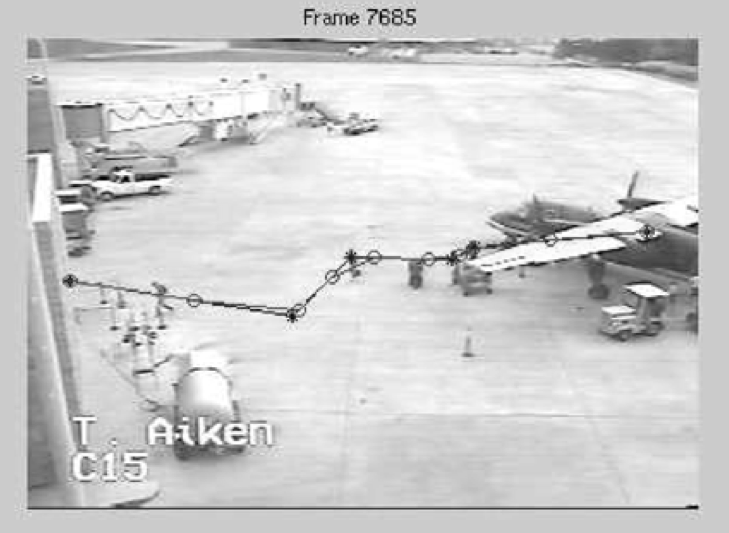
\includegraphics[width=2in]{figures/vaswani-abnormal-activity.png}}
%    \caption[Vaswani et al.'s experimental results on an airport scenario.]
%        {\small Vaswani et al.'s 
%        experimental results on an airport scenario. (a) A ``normal activity'' 
%        frame with 4 people. 
%        (b) Abnormality introduced by making one person walk-away in an 
%        abnormal direction. Reprinted from Vaswani et al.\ (2005)}
%    \label{fig:vaswani-work}
%\end{figure}

\section{Contributions}

The contributions of this dissertation are as follows.

\begin{enumerate}
  \item We propose an intelligent video surveillance system that is
    practical and fairly close to the ideal surveillance system, which
    should monitor activity and automatically trigger alarms to security
    personnel;

  \item We develop an algorithm for extracting and tracking multiple 
    moving foreground blobs in a scene using an appearance model;

  \item We propose a shadow detection method that uses a simple
    maximum likelihood classification approach based on color
    information;

  \item We propose a new method for clustering human behaviors that 
    is suitable for bootstrapping an anomaly detection module for 
    intelligent video surveillance systems;

  \item We propose and develop a new and effective algorithm for
    semi-supervised learning of common human behaviors and detect 
    anomalies in video sequences;

  \item We introduce a new and more accurate algorithm for
    incrementally profiling human behaviors in video sequences without
    requiring storage of large databases of training data;

  \item We provide the source code and datasets
    online\footnote{See \url{http://www.kanouivirach.com/#downloads}.}
    for researchers interested in evaluating or extending our work.
\end{enumerate}

\subsection{List of Publications}

We provide a list of publications as part of this dissertation. We
also include the list of works currently under review and preparation
for submission.

\subsection*{Published Works}

\begin{itemize}
  \renewcommand\labelitemi{--} 
  
  \item {\bf{Extracting the Object from the Shadows: Maximum
    Likelihood Object/Shadow Discrimination}}\\ Kan Ouivirach and
    Matthew N.\ Dailey\\ \textit{International Conference on
    Electrical Engineering/Electronics Computer Telecommunications and
    Information Technology (ECTI-CON)}, pages 1--5, 2013\\ 
    Publisher: IEEE Computer Society\\ Included in 
    Chapter~\ref{ch:shadow}

  \item \textbf{Clustering Human Behaviors with Dynamic Time Warping
    and Hidden Markov Models for a Video Surveillance
    System}\nocite{kan10clustering}\\ Kan Ouivirach and Matthew N.\
    Dailey\\ \textit{International Conference on Electrical
    Engineering/Electronics Computer Telecommunications and
    Information Technology (ECTI-CON)}, pages 884--888, 2010\\
    Publisher: IEEE Computer Society\\ Included in
    Chapter~\ref{ch:clustering}\\

  \item \textbf{Automatic Suspicious Behavior Detection from a Small
    Bootstrap Set}\nocite{kan12detection}\\ Kan Ouivirach, Shashi
    Gharti, and Matthew N.\ Dailey\\ \textit{International Conference
    on Computer Vision Theory and Applications (VISAPP)}, volume 1,
    pages 655--658, 2012\\ Publisher: Springer-Verlag\\ Included in
    Chapter~\ref{ch:batch}\\

  \item \textbf{Incremental Behavior Modeling and Suspicious Activity
    Detection}\nocite{kan13incremental}\\ Kan Ouivirach, Shashi
    Gharti, and Matthew N.\ Dailey\\ \textit{Pattern Recognition},
    46(3): 671--680, 2013\\ Publisher: Elsevier\\ Included in
    Chapter~\ref{ch:incremental}
  
\end{itemize}

\subsection*{Manuscripts Currently in Preparation}

\begin{itemize}
  \renewcommand\labelitemi{--}

  \item {\bf{Incorporating Geometric and Shadow Region Shape
    Information for Shadow Detection}}\\ Kan Ouivirach and Matthew N.\
    Dailey\\ To be submitted in \textit{International Conference on
    Computer Vision and Pattern Recognition (CVPR)}, 2013\\ Publisher:
    IEEE Computer Society

\end{itemize}

\section{Organization of Dissertation}

I organize the rest of this dissertation as follows.

In Chapter \ref{ch:blobanalysis}, I describe our blob-based motion
analysis methods including blob extraction and appearance-based blob
tracking.

In Chapter \ref{ch:shadow}, I present a new method for detecting
shadows using a simple maximum likelihood classification method based
on color information.

In Chapter \ref{ch:clustering}, I propose a new method for clustering
behaviors in a scene.

In Chapter \ref{ch:batch}, I present an automatic suspicious behavior
detection method that uses a small bootstrap set.

In Chapter \ref{ch:incremental}, I describe our extension of the
suspicious behavior detection approach for incremental learning in
which security personnel feedback is incorporated.

Finally, in Chapter \ref{ch:conclusion}, I conclude and discuss the
possible further extensions of my dissertation.

\FloatBarrier


% --- Maybe use later ---

%(see Figure \ref{fig:zm-console}) 
%\begin{figure}[t]
%  \begin{center}
%    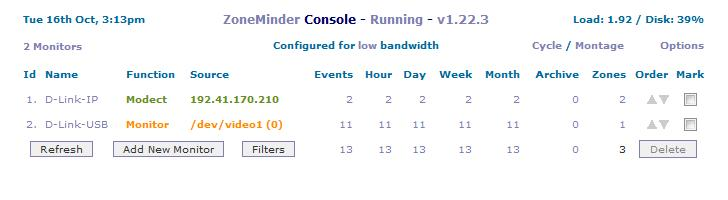
\includegraphics[width=4.5in]{figures/zm-console.jpg}
%    \caption{ZM Console} 
%    \label{fig:zm-console}
%  \end{center}
%\end{figure}

%ZM has three main modules. The first is the ZM Capture (ZMC) module
%whose job is to capture video frames from a video device as quickly as
%possible. The second is the ZM Analysis (ZMA) module, which performs
%video analysis. It finds the captured frames and checks whether the
%detected motion should generate an alarm or not. The last is the ZM
%Frame (ZMF) module. It is an optional module for writing the captured
%frames to file system. This module could potentially reduce the
%workload of ZMA, so ZMA can do more analysis work. If ZMF is not
%enabled, ZMA will write captured frames to file system instead.

%The core of ZM supports capturing and analyzing images. It also
%provides a configurable set of parameters (see
%Figure \ref{fig:zm-option}). ZM allows us to define ``zones'' for each
%camera and vary the sensitivity and functionality (see
%Figure \ref{fig:zm-webcam01-zones}
%and \ref{fig:zm-webcam01-zones-define}). Therefore, we can eliminate
%unnecessary regions and set the different thresholds for each zone. ZM
%also provides a motion detection feature for detecting changes in a
%scene and setting an alarm based on the user-defined threshold.

%\begin{figure}[t]
%  \begin{center}
%    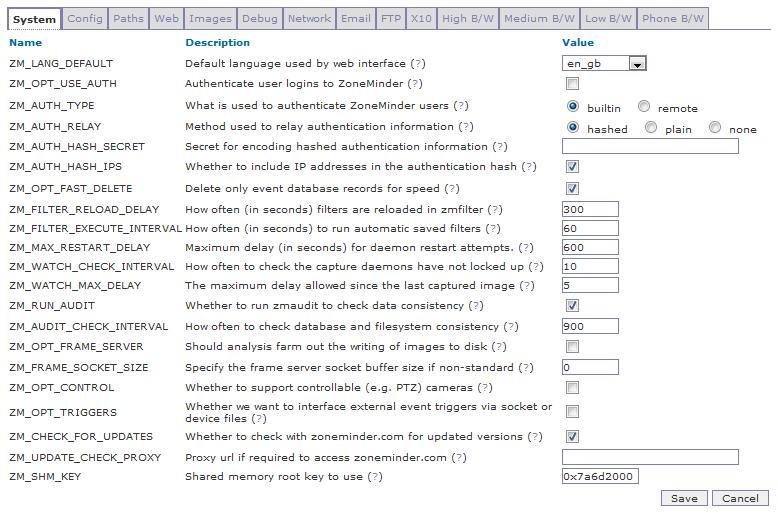
\includegraphics[width=4.5in]{figures/zm-options.jpg}
%    \caption{ZM Options}
%    \label{fig:zm-option}
%  \end{center}
%\end{figure}

%\begin{figure}[t]
%  \begin{center}
%    \subfloat[]{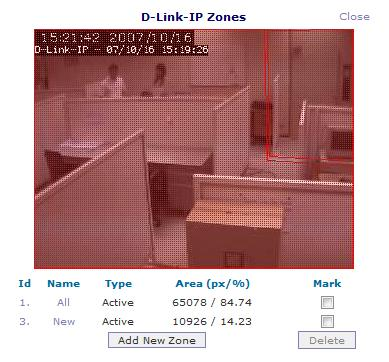
\includegraphics[scale=0.5]{figures/zm-webcam01-zones.jpg}\label{fig:zm-webcam01-zones}}
%    \hspace{0.1in}
%    \subfloat[]{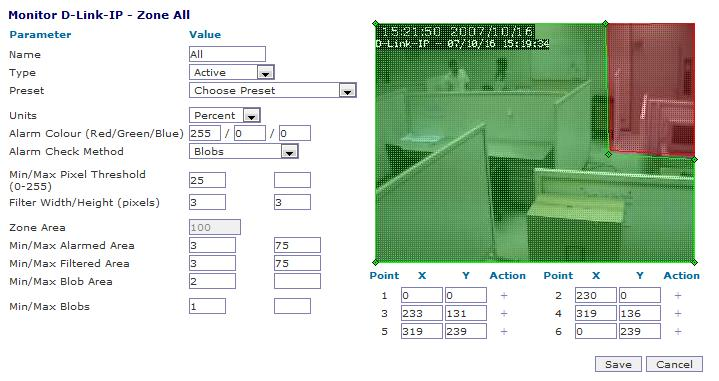
\includegraphics[scale=0.5]{figures/zm-webcam01-zones-define.jpg}\label{fig:zm-webcam01-zones-define}}
%  \end{center}  
%  \caption[Example of zone defined in ZoneMinder]{Example of (a) zone
%  defined and (b) configuring a zone in ZoneMinder.}
%  \label{fig:zm-webcam-zones}
%\end{figure}

%Here I review only the intrusion detection module.  
%The intrusion detection module automatically detects prohibited
%intrusion behaviors while ignoring distractions that cause false
%alarms, like small animals, swaying branches,
%etc. Figure \ref{fig:intrusion-detection} shows a screen shot of the
%result from this module. This module can be used on stationary cameras
%as well as on PTZ cameras. There are two modes which are Regional
%Entrance and Tripwire. The first mode provides a security alarm when
%the system detects a person or vehicle moving within a prohibited
%area. The second mode provides a security alarm when a person or
%vehicle breaks through a demarcation line. User can configure this
%mode to prohibit any crossover or to allow movement in a single
%direction.

%\begin{figure}[t]
%  \begin{center}
%    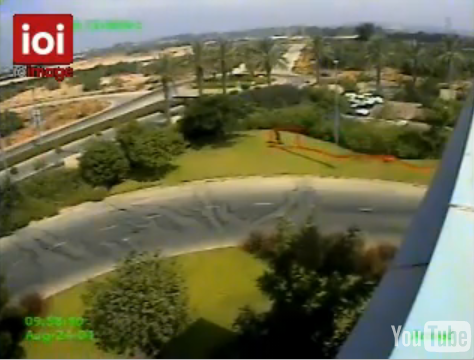
\includegraphics[width=3in]{figures/intrusion-detection.png}
%     \caption[Screen shot of DVTel's intrusion detection
%     module]{Screen shot of DVTel's intrusion detection
%     module. Captured from the video demonstration on DVTel's Web
%     site.}
%    \label{fig:intrusion-detection}
%  \end{center}
%\end{figure}

%For example, it has the knowledge that a head contains two
%eyes and a mouth; so, if either an eye or mouth is detected, it will
%assume that there is a head at that position. Vitamin D Video trained
%a learning network with several hundred videos of humans. Also,
%examples of vehicles and animals not people are trained. As a result,
%Vitamin D Video can tolerate to real world problems.

